\chapter{Inside the Atom}\label{ch:g9:inside-the-atom}

In 1909, in a laboratory in Manchester, a beam of tiny, fast particles
was fired at a sheet of gold leaf a few hundred \omterm{def:g7:atoms-and-molecules:atom}{atoms} thick. Nearly all
of them went straight through, as if the gold were empty. But about one
in several thousand bounced back. ``It was as if you fired a 15-inch
shell at a piece of tissue paper and it came back and hit you,'' said
Ernest Rutherford, whose students had made the experiment. The \omterm{def:g7:atoms-and-molecules:atom}{atom},
the uncuttable piece of matter, had a structure --- and it was almost
entirely empty.

\begin{recall}
All matter is made of \omterm{def:g7:atoms-and-molecules:atom}{atoms}, about a hundred different kinds of them,
each with a symbol such as \ce{H}, \ce{C}, \ce{O}, \ce{Fe}. \omterm{def:g7:atoms-and-molecules:atom}{Atoms} join
into \omterm{def:g7:atoms-and-molecules:molecule}{molecules}, described by formulas such as \ce{H2O}
(\cref{ch:g7:atoms-and-molecules}).
\end{recall}

\section{Nucleus and electrons}

\begin{definition}[Nucleus and electron]\label{def:g9:inside-the-atom:nucleus}
Every \omterm{def:g7:atoms-and-molecules:atom}{atom} has a tiny, heavy core, the \emph{nucleus}\index{nucleus},
which carries a positive electric charge. Around it move much lighter
particles, the \emph{electrons}\index{electron}, each carrying the same
negative charge, $-e$.
\end{definition}

\begin{proposition}[An atom is neutral]\label{prop:g9:inside-the-atom:neutral}
% ledger: const:e
An \omterm{def:g7:atoms-and-molecules:atom}{atom} as a whole carries no electric charge: the positive charge of its
\omterm{def:g9:inside-the-atom:nucleus}{nucleus} is exactly balanced by the negative charges of its \omterm{def:g9:inside-the-atom:nucleus}{electrons}.
The charge $e$ is tiny: $e = \qty{1.60e-19}{C}$ (the coulomb, unit of
charge, is the physics book's).
\end{proposition}

\begin{omfigure}
\begin{tikzpicture}[font=\small]
  \shade[inner color=omDef!35, outer color=white] (0,0) circle (2.2);
  \draw[omDef!60, dashed] (0,0) circle (2.2);
  \foreach \a/\r in {20/1.6,95/1.1,150/1.9,215/1.4,290/1.7,340/0.9} {
    \fill[omDef] (\a:\r) circle (0.06);
    \node[font=\scriptsize, omDef] at ($(\a:\r)+(0.18,0.16)$) {$-$};
  }
  \fill[red!70!black] (0,0) circle (0.1);
  \draw[<-, omProp, thick] (-0.12,0.02) -- (-3.0,0.9) node[left, text=black, align=right]
    {nucleus: tiny,\\ heavy, positive};
  \draw[<-, omProp, thick] ($(20:1.6)+(0.08,0.02)$) -- (3.0,0.9) node[right, text=black]
    {an electron: light, negative};
  \draw[<-, omProp, thick] (300:2.2) -- (3.0,-1.4) node[right, text=black, align=left]
    {the electrons move in a cloud\\ around the nucleus};
\end{tikzpicture}

{\small An \omterm{def:g7:atoms-and-molecules:atom}{atom}, not to scale. If the \omterm{def:g9:inside-the-atom:nucleus}{nucleus} were drawn the size of the
red dot, the cloud of \omterm{def:g9:inside-the-atom:nucleus}{electrons} would be a few hundred metres across.}
\end{omfigure}

\section{Protons and neutrons}

\begin{definition}[Proton, neutron, nucleon]\label{def:g9:inside-the-atom:proton}
The \omterm{def:g9:inside-the-atom:nucleus}{nucleus} is made of two kinds of particles: \emph{protons}\index{proton},
each carrying the charge $+e$, and \emph{neutrons}\index{neutron},
which carry no charge. Protons and neutrons, which have almost the same
mass, are together called \emph{nucleons}\index{nucleon}.
\end{definition}

\begin{definition}[Atomic number and mass number]\label{def:g9:inside-the-atom:atomic-number}
The number of \omterm{def:g9:inside-the-atom:proton}{protons} in a \omterm{def:g9:inside-the-atom:nucleus}{nucleus} is the \emph{atomic
number}\index{atomic number}, written $Z$. The number of \omterm{def:g9:inside-the-atom:proton}{nucleons}
(\omterm{def:g9:inside-the-atom:proton}{protons} and \omterm{def:g9:inside-the-atom:proton}{neutrons} together) is the \emph{mass number}\index{mass
number}, written $A$. The number of \omterm{def:g9:inside-the-atom:proton}{neutrons} is $N = A - Z$.
\end{definition}

\begin{notation}[The nuclide symbol]\label{not:g9:inside-the-atom:symbol}
An \omterm{def:g7:atoms-and-molecules:atom}{atom} with a given \omterm{def:g9:inside-the-atom:nucleus}{nucleus} is written with its symbol, the \omterm{def:g9:inside-the-atom:atomic-number}{mass number}
at the top left and the \omterm{def:g9:inside-the-atom:atomic-number}{atomic number} at the bottom left:
\ce{^{A}_{Z}X}. For example \ce{^{12}_{6}C} has 6 \omterm{def:g9:inside-the-atom:proton}{protons} and $12 - 6 =
6$ \omterm{def:g9:inside-the-atom:proton}{neutrons}; \ce{^{56}_{26}Fe} has 26 \omterm{def:g9:inside-the-atom:proton}{protons} and 30 \omterm{def:g9:inside-the-atom:proton}{neutrons}.
\end{notation}

\begin{method}[Reading a nuclide symbol]\label{met:g9:inside-the-atom:read}
For \ce{^{A}_{Z}X}:
\begin{enumerate}
  \item \omterm{def:g9:inside-the-atom:proton}{protons}: $Z$;
  \item \omterm{def:g9:inside-the-atom:proton}{neutrons}: $A - Z$;
  \item \omterm{def:g9:inside-the-atom:nucleus}{electrons} of the neutral \omterm{def:g7:atoms-and-molecules:atom}{atom}: $Z$, the same as the \omterm{def:g9:inside-the-atom:proton}{protons}.
\end{enumerate}
For \ce{^{23}_{11}Na}: 11 \omterm{def:g9:inside-the-atom:proton}{protons}, 12 \omterm{def:g9:inside-the-atom:proton}{neutrons}, 11 \omterm{def:g9:inside-the-atom:nucleus}{electrons}.
\end{method}

\begin{omfigure}
\begin{tikzpicture}[font=\small]
  \node[font=\Huge, inner sep=1pt] (x) at (0,0) {\ce{^{35}_{17}Cl}};
  \draw[<-, omProp, thick, shorten <=3pt] ([xshift=5pt,yshift=-7pt]x.north west) -- (-2.6,1.0)
    node[left, text=black, align=right] {mass number $A = 35$:\\ protons + neutrons};
  \draw[<-, omProp, thick, shorten <=3pt] ([xshift=5pt,yshift=7pt]x.south west) -- (-2.6,-1.0)
    node[left, text=black, align=right] {atomic number $Z = 17$:\\ protons};
  \draw[<-, omProp, thick] ([xshift=2pt]x.east) -- (2.2,0) node[right, text=black,
    align=left] {symbol of the element:\\ chlorine};
\end{tikzpicture}

{\small Reading a nuclide symbol: this chlorine \omterm{def:g7:atoms-and-molecules:atom}{atom} has 17 \omterm{def:g9:inside-the-atom:proton}{protons},
$35 - 17 = 18$ \omterm{def:g9:inside-the-atom:proton}{neutrons}, and 17 \omterm{def:g9:inside-the-atom:nucleus}{electrons} when neutral.}
\end{omfigure}

\section{The chemical element and its isotopes}

\begin{definition}[Chemical element]\label{def:g9:inside-the-atom:element}
A \emph{chemical element}\index{chemical element} is the set of all the
\omterm{def:g7:atoms-and-molecules:atom}{atoms}, and of all the charged \omterm{def:g7:atoms-and-molecules:atom}{atoms} made from them, that have the same
\omterm{def:g9:inside-the-atom:atomic-number}{atomic number} $Z$. Each element has a name and a symbol: every \omterm{def:g7:atoms-and-molecules:atom}{atom} with
6 \omterm{def:g9:inside-the-atom:proton}{protons} is a carbon \omterm{def:g7:atoms-and-molecules:atom}{atom}, \ce{C}; every \omterm{def:g7:atoms-and-molecules:atom}{atom} with 8 \omterm{def:g9:inside-the-atom:proton}{protons} is an
oxygen \omterm{def:g7:atoms-and-molecules:atom}{atom}, \ce{O}.
\end{definition}

\begin{definition}[Isotopes]\label{def:g9:inside-the-atom:isotope}
\omterm{def:g7:atoms-and-molecules:atom}{Atoms} of the same element that have different numbers of \omterm{def:g9:inside-the-atom:proton}{neutrons}, and
so different \omterm{def:g9:inside-the-atom:atomic-number}{mass numbers}, are \emph{isotopes}\index{isotope} of that
element. They have the same $Z$ and different $A$.
\end{definition}

\begin{example}[Isotopes of carbon and of hydrogen]\label{ex:g9:inside-the-atom:isotopes}
% ledger: iso:C12, iso:C13, iso:H2
Natural carbon is about \qty{98.9}{\percent} carbon-12, \ce{^{12}_{6}C},
and \qty{1.1}{\percent} carbon-13, \ce{^{13}_{6}C}, with a trace of
carbon-14, \ce{^{14}_{6}C}, whose slow change into another \omterm{def:g9:inside-the-atom:nucleus}{nucleus} is
used to date ancient wood and bones (radioactivity belongs to the
physics book). Hydrogen has three \omterm{def:g9:inside-the-atom:isotope}{isotopes}: \ce{^{1}_{1}H}, with no
\omterm{def:g9:inside-the-atom:proton}{neutron} at all, the commonest by far; deuterium \ce{^{2}_{1}H}, a few
\omterm{def:g7:atoms-and-molecules:atom}{atoms} in every hundred thousand; and tritium \ce{^{3}_{1}H}.
\end{example}

\begin{proposition}[Isotopes behave alike in chemistry]\label{prop:g9:inside-the-atom:alike}
The chemistry of an \omterm{def:g7:atoms-and-molecules:atom}{atom} depends on its \omterm{def:g9:inside-the-atom:nucleus}{electrons}, and the \omterm{def:g9:inside-the-atom:isotope}{isotopes} of
an element have the same number of \omterm{def:g9:inside-the-atom:nucleus}{electrons}. \omterm{def:g9:inside-the-atom:isotope}{Isotopes} therefore react
in the same way: water made with deuterium looks and behaves almost
exactly like ordinary water.
\end{proposition}

\begin{omfigure}
\begin{tikzpicture}[font=\small, p/.style={circle, inner sep=0pt, minimum size=4.2mm,
    ball color=red!65}, n/.style={circle, inner sep=0pt, minimum size=4.2mm,
    ball color=black!20}]
  \node[p] at (0,0) {};
  \node[anchor=north, align=center] at (0,-0.45) {\ce{^{1}_{1}H}\\ 1 proton};
  \node[p] at (3.0,0) {}; \node[n] at (3.35,0.1) {};
  \node[anchor=north, align=center] at (3.2,-0.45) {\ce{^{2}_{1}H}\\ 1 proton, 1 neutron};
  \node[p] at (6.4,0) {}; \node[n] at (6.75,0.12) {}; \node[n] at (6.55,0.35) {};
  \node[anchor=north, align=center] at (6.6,-0.45) {\ce{^{3}_{1}H}\\ 1 proton, 2 neutrons};
  \node[draw=black!30, fill=red!65, circle, minimum size=3mm, inner sep=0pt] at (9.1,0.2) {};
  \node[anchor=west] at (9.3,0.2) {proton};
  \node[draw=black!30, fill=black!20, circle, minimum size=3mm, inner sep=0pt] at (9.1,-0.3) {};
  \node[anchor=west] at (9.3,-0.3) {neutron};
\end{tikzpicture}

{\small The nuclei of the three \omterm{def:g9:inside-the-atom:isotope}{isotopes} of hydrogen: one \omterm{def:g9:inside-the-atom:proton}{proton} each,
and 0, 1 or 2 \omterm{def:g9:inside-the-atom:proton}{neutrons}.}
\end{omfigure}

\section{Sizes and masses}

\begin{proposition}[The nucleus is tiny and holds almost all the mass]\label{prop:g9:inside-the-atom:sizes}
% ledger: const:a0, r:proton, const:mp, const:mn, const:me
An \omterm{def:g7:atoms-and-molecules:atom}{atom} measures about \qty{e-10}{m} across; its \omterm{def:g9:inside-the-atom:nucleus}{nucleus}, about
\qty{e-15}{m} to \qty{e-14}{m}: some ten thousand to a hundred thousand
times smaller. The masses of the particles are
\[
  m_p = \qty{1.673e-27}{kg},\qquad m_n = \qty{1.675e-27}{kg},\qquad
  m_e = \qty{9.11e-31}{kg}.
\]
A \omterm{def:g9:inside-the-atom:proton}{proton} is about 1836 times heavier than an \omterm{def:g9:inside-the-atom:nucleus}{electron}, so more than
\qty{99.9}{\percent} of the mass of an \omterm{def:g7:atoms-and-molecules:atom}{atom} is in its \omterm{def:g9:inside-the-atom:nucleus}{nucleus}.
\end{proposition}

\begin{example}[A marble in a stadium]\label{ex:g9:inside-the-atom:marble}
If the \omterm{def:g9:inside-the-atom:nucleus}{nucleus} of an \omterm{def:g7:atoms-and-molecules:atom}{atom} were a marble \qty{1}{cm} across, the \omterm{def:g7:atoms-and-molecules:atom}{atom}
would be about $\qty{1}{cm} \times 100\,000 = \qty{1}{km}$ across: a
marble in the middle of a huge stadium, with a few specks of dust ---
the \omterm{def:g9:inside-the-atom:nucleus}{electrons} --- whirling around the stands. Matter is mostly empty
space.
\end{example}

\begin{method}[The mass of an atom]\label{met:g9:inside-the-atom:mass}
Since \omterm{def:g9:inside-the-atom:proton}{protons} and \omterm{def:g9:inside-the-atom:proton}{neutrons} have nearly the same mass and \omterm{def:g9:inside-the-atom:nucleus}{electrons} are
very light, the mass of an \omterm{def:g7:atoms-and-molecules:atom}{atom} is close to $A \times
\qty{1.67e-27}{kg}$, where $A$ is its \omterm{def:g9:inside-the-atom:atomic-number}{mass number}. A carbon-12 \omterm{def:g7:atoms-and-molecules:atom}{atom}:
$12 \times 1.67 \times 10^{-27} = \qty{2.00e-26}{kg}$.
\end{method}

\section{A short history of the atomic model}

\begin{history}[From the uncuttable to the nucleus, 1897--1932]
In 1897 J.~J.~Thomson discovered the \omterm{def:g9:inside-the-atom:nucleus}{electron}, a particle far lighter
than any \omterm{def:g7:atoms-and-molecules:atom}{atom}: \omterm{def:g7:atoms-and-molecules:atom}{atoms} could be cut after all. He pictured the \omterm{def:g7:atoms-and-molecules:atom}{atom} as a
ball of positive matter studded with \omterm{def:g9:inside-the-atom:nucleus}{electrons}. In 1909--1911 the
gold-foil experiment of Rutherford's team showed that the positive
charge and almost all the mass sit in a tiny \omterm{def:g9:inside-the-atom:nucleus}{nucleus}. In 1913 Niels
Bohr proposed that the \omterm{def:g9:inside-the-atom:nucleus}{electrons} occupy fixed energy levels around it,
and in 1932 James Chadwick found the \omterm{def:g9:inside-the-atom:proton}{neutron}.
\end{history}

\begin{omfigure}
\begin{minipage}[b]{0.3\linewidth}\centering
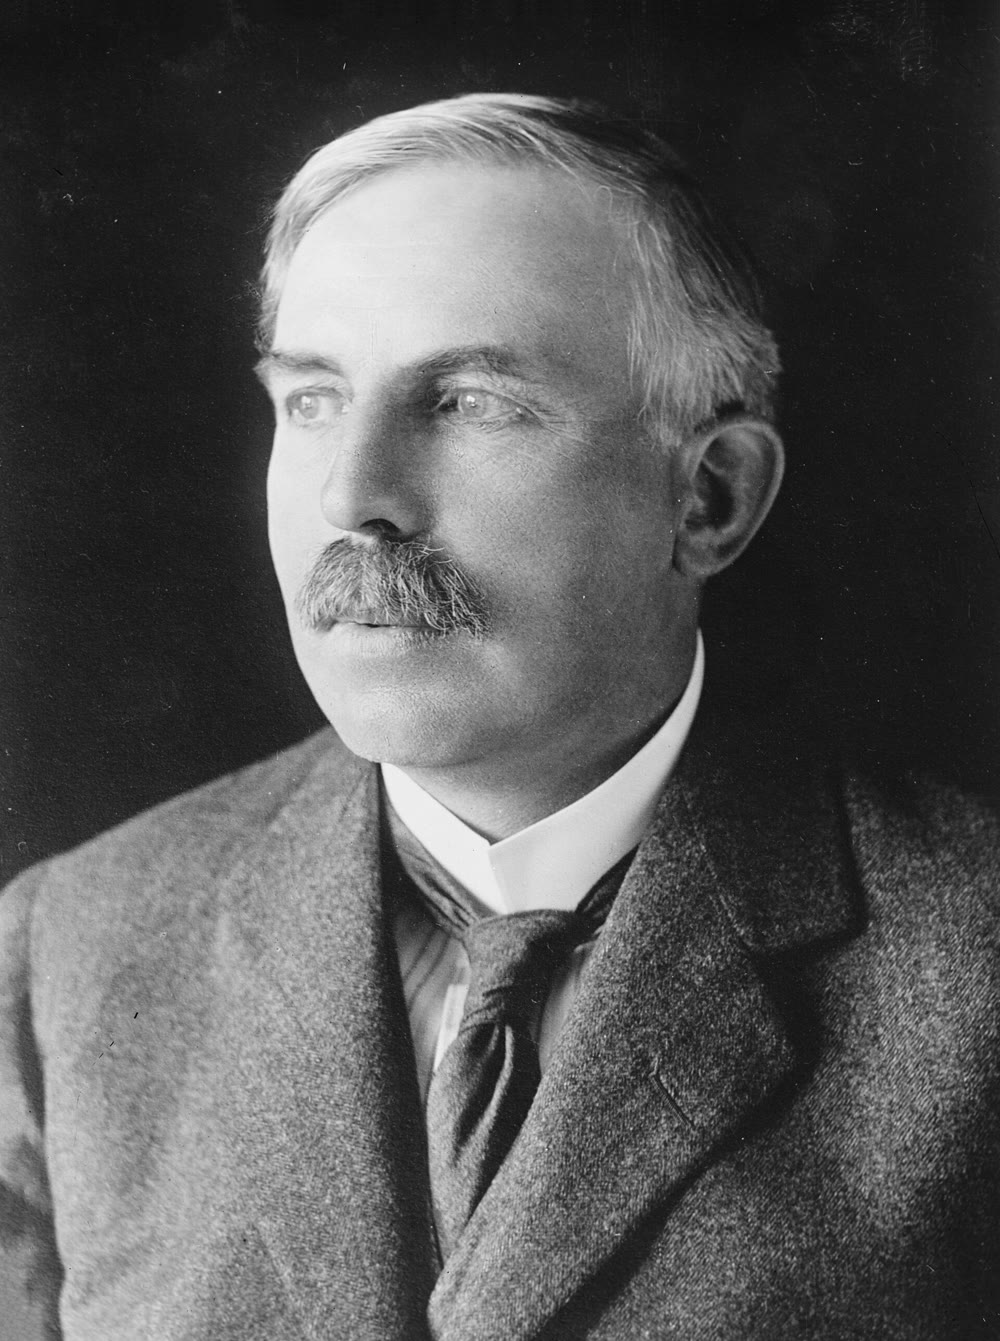
\includegraphics[width=\linewidth]{images/book1/rutherford.jpg}

{\small Ernest Rutherford (1871--1937).}
\end{minipage}\hfill
\begin{minipage}[b]{0.66\linewidth}\centering
\begin{tikzpicture}[font=\small]
  \fill[black!45] (0,-0.5) rectangle (0.9,0.5);
  \node[anchor=north, align=center] at (0.45,-0.55) {source of\\ alpha particles};
  \draw[->, thick, red!70!black] (0.9,0) -- (2.8,0);
  \fill[yellow!70!orange] (2.8,-1.6) rectangle (2.88,1.6);
  \node[anchor=north] at (2.84,-1.65) {gold leaf};
  \draw[omDef!40, line width=4pt] (5.6,-1.8) arc[start angle=-30, end angle=30, radius=3.6];
  \foreach \y in {-0.3,-0.1,0.1,0.3} \draw[->, red!70!black] (2.88,\y) -- (5.3,\y);
  \draw[->, red!70!black] (2.88,0.05) -- (5.0,1.15);
  \draw[->, red!70!black] (2.88,-0.05) -- (4.9,-1.3);
  \draw[->, red!70!black, thick] (2.8,0.02) .. controls (2.2,0.35) .. (1.6,0.95);
  \node[anchor=west, align=left, font=\footnotesize] at (6.25,0) {most go\\ straight\\ through};
  \node[anchor=south, align=center, font=\footnotesize] at (1.6,1.0) {a very few\\ bounce back};
\end{tikzpicture}

{\small The gold-foil experiment: most particles pass straight through;
a few are deflected; a very few bounce back from a \omterm{def:g9:inside-the-atom:nucleus}{nucleus}.}
\end{minipage}
\end{omfigure}

\section{Exercises}

\begin{exercise}[$\star$]\label{exo:g9:inside-the-atom:1}
Name the particles of the \omterm{def:g9:inside-the-atom:nucleus}{nucleus} and the particles around it, with the
sign of their charge.
\end{exercise}

\begin{exercise}[$\star$]\label{exo:g9:inside-the-atom:2}
Give the number of \omterm{def:g9:inside-the-atom:proton}{protons}, \omterm{def:g9:inside-the-atom:proton}{neutrons} and \omterm{def:g9:inside-the-atom:nucleus}{electrons} of \ce{^{16}_{8}O},
\ce{^{27}_{13}Al} and \ce{^{40}_{20}Ca}.
\end{exercise}

\begin{exercise}[$\star$]\label{exo:g9:inside-the-atom:3}
Why is an \omterm{def:g7:atoms-and-molecules:atom}{atom} electrically neutral?
\end{exercise}

\begin{exercise}[$\star$]\label{exo:g9:inside-the-atom:4}
An \omterm{def:g7:atoms-and-molecules:atom}{atom} has 26 \omterm{def:g9:inside-the-atom:proton}{protons} and 30 \omterm{def:g9:inside-the-atom:proton}{neutrons}. Write its nuclide symbol (the
element is iron, \ce{Fe}).
\end{exercise}

\begin{exercise}[$\star\star$]\label{exo:g9:inside-the-atom:5}
Are \ce{^{35}_{17}Cl} and \ce{^{37}_{17}Cl} the same element? Are they
\omterm{def:g9:inside-the-atom:isotope}{isotopes}? Explain.
\end{exercise}

\begin{exercise}[$\star\star$]\label{exo:g9:inside-the-atom:6}
Are \ce{^{14}_{6}C} and \ce{^{14}_{7}N} \omterm{def:g9:inside-the-atom:isotope}{isotopes}? Explain.
\end{exercise}

\begin{exercise}[$\star\star$]\label{exo:g9:inside-the-atom:7}
Compute, in scientific notation, the approximate mass of an \omterm{def:g7:atoms-and-molecules:atom}{atom} of
\ce{^{56}_{26}Fe}.
\end{exercise}

\begin{exercise}[$\star\star$]\label{exo:g9:inside-the-atom:8}
In the gold-foil experiment, why do most particles go straight through
the gold?
\end{exercise}

\begin{exercise}[$\star\star$]\label{exo:g9:inside-the-atom:9}
How many times smaller than an \omterm{def:g7:atoms-and-molecules:atom}{atom} (\qty{e-10}{m}) is a \omterm{def:g9:inside-the-atom:nucleus}{nucleus} of
\qty{e-15}{m}? Write the answer as a power of ten.
\end{exercise}

\begin{exercise}[$\star\star$]\label{exo:g9:inside-the-atom:10}
Why do the \omterm{def:g9:inside-the-atom:isotope}{isotopes} of an element have the same chemistry?
\end{exercise}

\begin{exercise}[$\star\star\star$]\label{exo:g9:inside-the-atom:11}
An iron \omterm{def:g7:atoms-and-molecules:atom}{atom} has 26 \omterm{def:g9:inside-the-atom:nucleus}{electrons}. Compute their total mass, then the
fraction of the mass of a \ce{^{56}_{26}Fe} \omterm{def:g7:atoms-and-molecules:atom}{atom} that they make up (use
the mass found in exercise~7).
\end{exercise}

\begin{exercise}[$\star\star\star$]\label{exo:g9:inside-the-atom:12}
% ledger: iso:Cu63, iso:Cu65
Natural copper is \qty{69.15}{\percent} copper-63 and \qty{30.85}{\percent}
copper-65. Among 10\,000 copper \omterm{def:g7:atoms-and-molecules:atom}{atoms}, how many are of each \omterm{def:g9:inside-the-atom:isotope}{isotope}?
What is the average number of \omterm{def:g9:inside-the-atom:proton}{nucleons} per copper \omterm{def:g7:atoms-and-molecules:atom}{atom}?
\end{exercise}

\clearpage % keeps the heading with its problem box (it was stranded at a page foot)
\section{Problem: Weighing Chlorine}

\begin{problem}[{Weekend problem --- two isotopes of chlorine, the mass
of each atom, and the average mass of a chlorine atom}]
\label{pb:g9:inside-the-atom:1}
% ledger: iso:Cl35, iso:Cl37, const:me, const:mp, const:mn
Natural chlorine is a \omterm{def:g6:pure-substances-and-mixtures:mixture}{mixture} of two \omterm{def:g9:inside-the-atom:isotope}{isotopes}, chlorine-35 and
chlorine-37: out of 1000 chlorine \omterm{def:g7:atoms-and-molecules:atom}{atoms}, about 758 are chlorine-35 and
242 chlorine-37. Take the mass of a \omterm{def:g9:inside-the-atom:proton}{nucleon} as \qty{1.67e-27}{kg} and
the mass of an \omterm{def:g9:inside-the-atom:nucleus}{electron} as \qty{9.11e-31}{kg}. The \omterm{def:g9:inside-the-atom:atomic-number}{atomic number} of
chlorine is 17.

\medskip
\noindent\textbf{Part I --- Two nuclei.}
\begin{enumerate}
  \item Write the nuclide symbols of the two \omterm{def:g9:inside-the-atom:isotope}{isotopes}.
  \item Give the number of \omterm{def:g9:inside-the-atom:proton}{protons}, \omterm{def:g9:inside-the-atom:proton}{neutrons} and \omterm{def:g9:inside-the-atom:nucleus}{electrons} of each.
  \item Why are both called chlorine? Why are they \omterm{def:g9:inside-the-atom:isotope}{isotopes}?
  \item Will a sample of chlorine-37 react with sodium the same way as a
        sample of chlorine-35? Explain.
\end{enumerate}

\medskip
\noindent\textbf{Part II --- The mass of each \omterm{def:g7:atoms-and-molecules:atom}{atom}.}
\begin{enumerate}[resume]
  \item Compute the mass of the \omterm{def:g9:inside-the-atom:nucleus}{nucleus} of a chlorine-35 \omterm{def:g7:atoms-and-molecules:atom}{atom}.
  \item Compute the mass of the 17 \omterm{def:g9:inside-the-atom:nucleus}{electrons}, and check that it can be
        neglected beside the \omterm{def:g9:inside-the-atom:nucleus}{nucleus}.
  \item Compute the mass of a chlorine-37 \omterm{def:g7:atoms-and-molecules:atom}{atom}.
  \item How many chlorine-35 \omterm{def:g7:atoms-and-molecules:atom}{atoms} would weigh \qty{1}{g}? Give the
        answer in scientific notation.
\end{enumerate}

\medskip
\noindent\textbf{Part III --- The average \omterm{def:g7:atoms-and-molecules:atom}{atom}.}
\begin{enumerate}[resume]
  \item What percentage of chlorine \omterm{def:g7:atoms-and-molecules:atom}{atoms} are chlorine-35? Chlorine-37?
  \item In 1000 \omterm{def:g7:atoms-and-molecules:atom}{atoms} of natural chlorine, compute the total mass of the
        chlorine-35 \omterm{def:g7:atoms-and-molecules:atom}{atoms} and of the chlorine-37 \omterm{def:g7:atoms-and-molecules:atom}{atoms}.
  \item Compute the mass of these 1000 \omterm{def:g7:atoms-and-molecules:atom}{atoms}.
  \item Deduce the average mass of a chlorine \omterm{def:g7:atoms-and-molecules:atom}{atom}.
\end{enumerate}
\end{problem}
